\subsection{Гипербола}
 
{\bfseries \term{Гипербола}} --- геометрическое место точек евклидовой плоскости, абсолютное значение разности расстояний от которых до двух выделенных точек $F_1$ и $F_2$, называемых фокусами, постоянно и равно удвоенной действительной полуоси гиперболы.
\begin{equation}
\bigl||F_1M|-|F_2M|\bigr| = 2a
\end{equation}

\begin{wrapfigure}[15]{r}{0.5\tw}
	\centering
	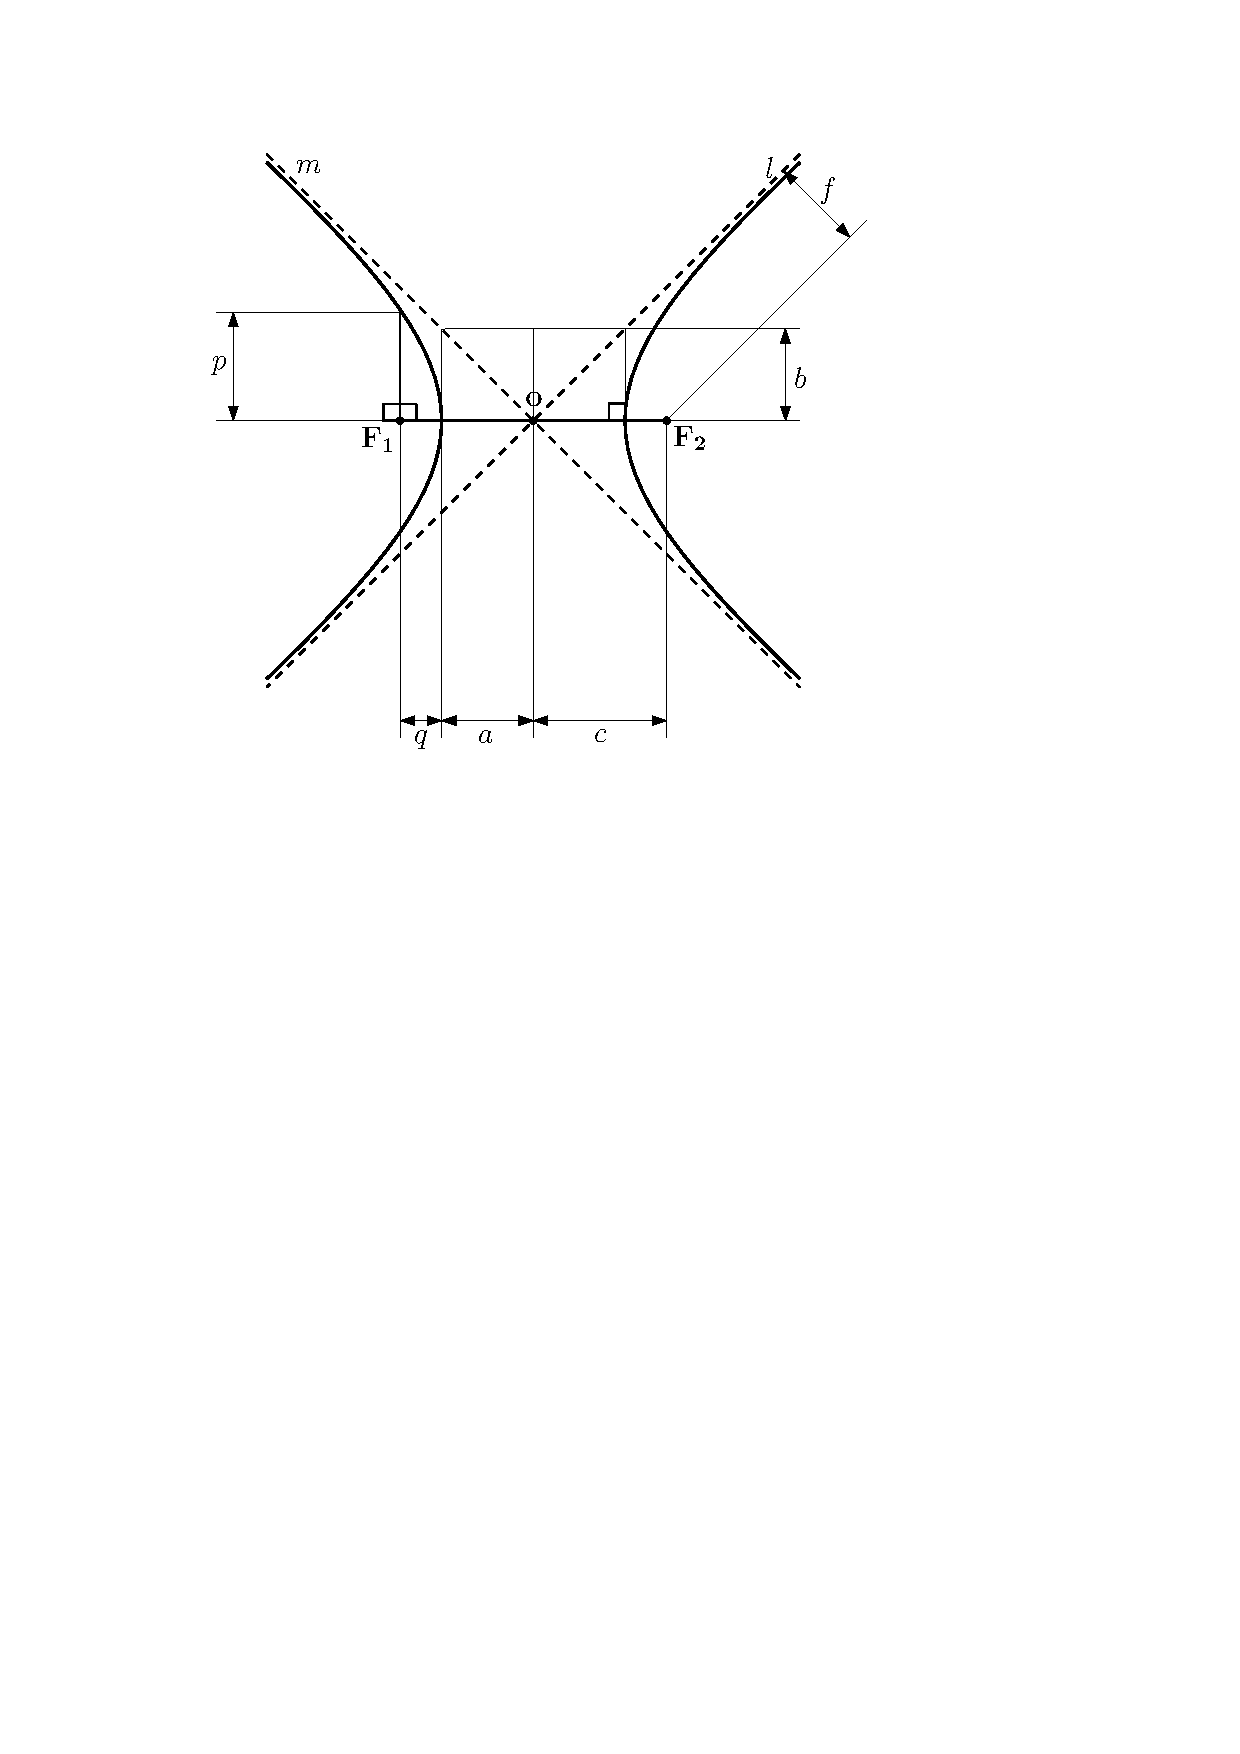
\includegraphics[width = 0.5\textwidth]{Hiperbola}
	\caption{Гипербола \label{pic:the-pic}}
\end{wrapfigure}
Ближайшие друг к другу точки двух ветвей гиперболы называются \term{вершинами} гиперболы. \term{Большая} или \term{действительная полуось}~($a$) гиперболы~--- расстояние от центра гиперболы до одной из вершин. \term{Фокальное расстояние}~($c$)~---  расстояние от центра гиперболы до одного из фокусов. \term{Эксцентриситетом} гиперболы~($e$), как и  эллипса, является отношение фокального расстояния к большой полуоси, так как большая полуось гиперболы всегда больше ее фокального расстояния, эксцентриситет гиперболы $e > 1$ и может быть найдет из определения:
\begin{equation}
e=\frac{c}{a}.
\end{equation}

\term{Перицентрическое расстояние} ($q$) --- расстояние от фокуса до ближайшей вершины гиперболы, можно найти, как
\begin{equation}
q = a ( e - 1).
\end{equation}

\term{Мнимая полуось}~($b$)~--- длина перпендикуляра к оси абсцисс, восставленного из вершины до пересечения с асимптотой. Равна \term{прицельному параметру}~($f$)~--- расстоянию от фокуса до асимптоты гиперболы.

\term{Фокальный параметр}~($p$)~--- длина отрезка, перпендикулярного к действительной оси, проведённого от фокуса до гиперболы. Определяется формулой
\begin{equation}
p=\frac{b^2}{a}.
\end{equation}

\imp{Каноническое уравнение гиперболы} в прямоугольных декартовых координатах записывается следующим образом:\begin{equation}
\frac{x^2}{a^2}-\frac{y^2}{b^2}=1.
\end{equation}

В \imp{полярных координатах} уравнение принимает вид:
\begin{equation}
r=\frac{p}{1-e\cos\varphi},
\end{equation}
причём полюс находится в фокусе гиперболы, а вершина гиперболы лежит на продолжении полярной оси.

\imp{Уравнение двух асимптот} является уравнением пересекающихся прямых:
\begin{equation}
	\frac{x}{a}\pm\frac{y}{b}=0.
\end{equation}

Важным соотношением для элементов гиперболы является
\begin{equation}
c^2=a^2+b^2.
\end{equation}

Также, как и любое коническое сечение, гипербола имеет своё {\itshape оптическое свойство}: свет от источника, находящегося в одном из фокусов гиперболы, отражается второй ветвью гиперболы таким образом, что продолжения отраженных лучей пересекаются во втором фокусе.
